\chapter{Introduction}
\label{chap:introduction}

\epigraph{
  Race de Caïn, au ciel monte,\\
  Et sur la terre jette Dieu !
}{---\textcite[16]{baudelaire-1857}}

%% \parencites[73]{elkins-2009}[49--50]{goguen-1991}[vii]{maclane-1998}[1,
%%   23]{marquis-2013}{nlab-category-theory}[xi]{pierce-1991}[415]{poigne-1992}[1154]{wolfram-2002}

Category theory is a branch of mathematics developed in the 1940s
which has come to occupy a central position in computer science.
Broadly, it is a convenient and powerful conceptual framework or
language for structures and systems of structures
\parencites[vii]{maclane-1998}[1]{marquis-2013}[1154]{wolfram-2002}.

In computer science, category theory allows us to formulate
definitions and theories, and to measure the elegance and coherence of
existing formulations, to carry out proofs, to discover and exploit
relations with other fields, to deal with abstraction and
representation independence, to formulate conjectures and research
directions, and to unify concepts \parencites[49--50]{goguen-1991}.
Additionally, category theory contributes to areas such as automata
theory, domain theory, functional programming, monads or notions of
computation, polymorphism, semantics, type theory, among others
\parencites[23]{marquis-2013}{nlab-category-theory}[xi]{pierce-1991}[415]{poigne-1992}.
In particular, category theory can be viewed as a formalization of
operations on data types, which provides a sound basis for functional
programming \parencites[414]{poigne-1992}[1154]{wolfram-2002}.

According to \textcite[73]{elkins-2009}, several concepts of
functional programming languages such as Haskell
\parencite{peytonjones-2003} and Agda \parencite{norell-2007} are
based on concepts of category theory, but one can be a perfectly
competent functional programmer without knowledge of these theoretical
foundations. In spite of that, category theory can be applied to
functional programming with the purpose of, for instance, better
understanding concepts such as algebraic data types, applicative
functors, functors, monads, and polymorphism, and thus becoming a
better programmer.

In this regard, we aim to explore the category-theoretical foundations
of some of the concepts of functional programming listed above. In
other words, we aim to see functional programming through category
theory.

\section*{Summary of the project}
\label{sec:introduction-summary}

This is an undergraduate project submitted in partial fulfillment of
the requirements for the degree of Systems Engineering at EAFIT
University\footnote{\url{http://www.eafit.edu.co}}. As a summary of
the project proposal, our objective is to study some of the
applications of category theory to functional programming in Haskell
and Agda. More specifically, our goal is to describe and explain the
concepts of category theory needed for conceptualizing and better
understanding algebraic data types, functors, monads, and
polymorphism.

\section*{Audience and prerequisites}
\label{sec:introduction-prerequisites}

The reader of this project is a mathematically inclined functional
programmer. We assume a working knowledge of mathematics and
functional programming in Haskell and Agda. If any further background
material is required, some suggestions can be found in the references
on page \pageref{sec:introduction-references} or in the references at
the end of each chapter.

\section*{Overview of the project}
\label{sec:introduction-overview}

\begin{figure}[htb]
  \begin{center}
    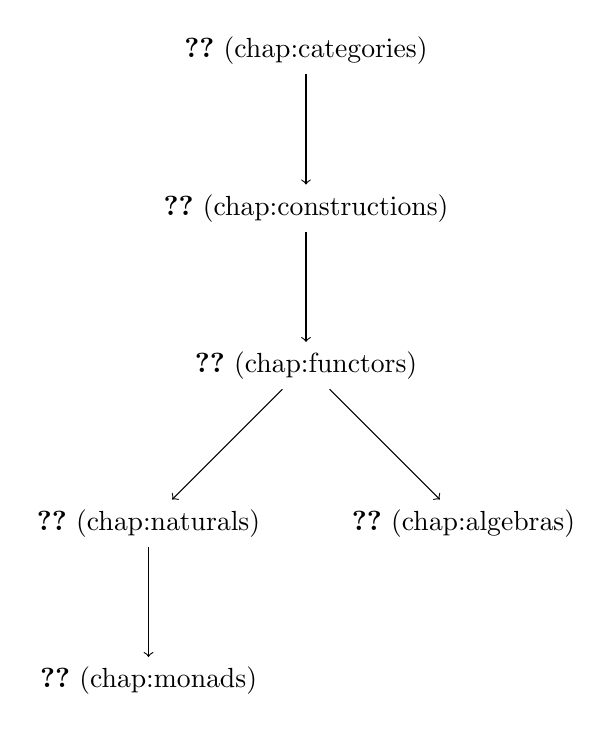
\begin{tikzpicture}
      \node (categories)    at (2,8) {\ref{chap:categories}    (\nameref{chap:categories})};
      \node (constructions) at (2,6) {\ref{chap:constructions} (\nameref{chap:constructions})};
      \node (functors)      at (2,4) {\ref{chap:functors}      (\nameref{chap:functors})};
      \node (naturals)      at (0,2) {\ref{chap:naturals}      (\nameref{chap:naturals})};
      \node (monads)        at (0,0) {\ref{chap:monads}        (\nameref{chap:monads})};
      \node (algebras)      at (4,2) {\ref{chap:algebras}      (\nameref{chap:algebras})};

      \draw [->] (categories)    to (constructions);
      \draw [->] (constructions) to (functors);

      \draw [->] (functors)      to (naturals);
      \draw [->] (naturals)      to (monads);

      \draw [->] (functors)      to (algebras);
    \end{tikzpicture}
  \end{center}
  \caption{Overview of the project.}
  \label{fig:overview}
\end{figure}

This project is divided into six chapters organized like the tree
diagram in Figure \ref{fig:overview}:
\begin{itemize}
\item
  In Chapter \ref{chap:categories} (\nameref{chap:categories}), we
  define categories and commutative diagrams, and the categories which
  will allow us to relate category theory to functional programming in
  Haskell and Agda.

\item
  In Chapter \ref{chap:constructions} (\nameref{chap:constructions}),
  we describe some basic constructions in categories (isomorphisms,
  initial and terminal objects, and products and coproducts), which we
  use for describing some concepts and examples in all subsequent
  chapters.

\item
  In Chapter \ref{chap:functors} (\nameref{chap:functors}), we study
  functors and endofunctors in order to conceptualize and better
  understand functors in Haskell and Agda.

\item
  In Chapter \ref{chap:naturals} (\nameref{chap:naturals}), we explore
  the connection between natural transformations and polymorphic
  functions in Haskell.

  This chapter completes the trinity of concepts category, functor,
  and natural transformation, which are the basis of category theory
  \parencite{nlab-category-theory}.

\item
  In Chapter \ref{chap:monads} (\nameref{chap:monads}), we give a
  detailed account of monads and Kleisli triples, and their
  correspondence to monads in Haskell and Agda.

\item
  In Chapter \ref{chap:algebras} (\nameref{chap:algebras}), we
  describe algebras and initial algebras over endofunctors, and their
  relation to algebraic data types in Haskell.

\item
  Finally, Chapter \ref{chap:conclusions} (\nameref{chap:conclusions})
  contains our conclusions and some ideas for future work.

\end{itemize}

Each chapter, except Chapter \ref{chap:constructions}, is further
subdivided into two or three sections concerning some concepts of
category theory, and their relation to functional programming in
Haskell and, in some cases, Agda. Additionally, each chapter ends with
a References section which collects the sources of information for all
definitions and examples.

\section*{References}
\label{sec:introduction-references}

This section includes a list of suggestions for further reading, as
well as some bibliographical remarks. For more thorough
category-theoretical reading guides, see
\parencites[48--56]{marquis-2013}[§ 4]{pierce-1991}.

\paragraph{Category theory}

\begin{itemize}
\item
  Most of our definitions are based on \parencite{maclane-1998}, which
  is the standard reference on category theory. However, it is a book
  for the working mathematician. On the other hand,
  \parencite{awodey-2010} is a book on category theory for anyone
  else.

\item
  \parencite{marquis-2013} includes an interesting description of the
  history of category theory, some of its applications, an analysis of
  its philosophical significance, and, perhaps more relevant, a useful
  programmatic reading guide.

\item
  As far as history is concerned, categories, functors, and natural
  transformations were discovered by
  \textcite{eilenberg-maclane-1942}, but category theory was devised
  in \parencite{eilenberg-maclane-1945}. Some of our definitions were
  compared with those of the latter.

\item
  \parencite{bird-demoor-1997} is a standard reference on the
  applications of category theory to computer science.

\item
  Some of our definitions and examples are based on
  \parencite{pierce-1991}, which covers the basic concepts of category
  theory and some of its applications to computer science. Besides, it
  includes a chapter with interesting reading suggestions.

\item
  Many of our definitions and some of our examples are based on
  \parencite{poigne-1992}, which is a complete reference on the
  applications of category theory to computer science.

\item
  Some works on category theory are not easily accessible.
  Fortunately, Reprints in Theory and Applications of
  Categories\footnote{\url{http://www.tac.mta.ca/tac/reprints/}}
  contains some interesting and useful books, including
  \parencites{adamek-et-al-2006}{barr-wells-2005}{barr-wells-2012}.

\item
  The $n$Lab\footnote{\url{http://ncatlab.org/nlab/}}, a wiki-lab for
  collaborative work on mathematics, physics, and philosophy, is a
  helpful source of information about category theory.

\end{itemize}

\paragraph{Haskell}

\begin{itemize}
\item
  Among the many tutorials on Haskell,
  \parencites{lipovaca-2011}{osullivan-et-al-2008} are highly
  recommended.

\item
  \parencite{yorgey-2009} is a nice introduction to the standard
  Haskell type classes, including categories, functors, and monads,
  and \parencite{elkins-2009} is an interesting article about how to
  use category theory in Haskell.

\item
  For more information, see the Haskell
  wiki\footnote{\url{http://www.haskell.org}}.

\end{itemize}

\paragraph{Agda}

\begin{itemize}
\item
  For an introduction to Agda, see
  \parencites{bove-dybjer-2009}{norell-2009}.

\item
  For more information, see the Agda
  wiki\footnote{\url{http://wiki.portal.chalmers.se/agda/}}.

\end{itemize}

\paragraph{Additional references}

\begin{itemize}
\item
  \parencite{weisstein-mathworld}, which is an extensive mathematics
  resource, was frequently consulted for supplementary information.

\item
  Some Stack Exchange\footnote{\url{http://stackexchange.com}} sites,
  notably MathOverflow and Stack Overflow, were consulted during the
  development of this project.

\end{itemize}

\section*{Notes}
\label{sec:introduction-notes}

\paragraph{Frontispiece}

The illustration in page \pageref{fig:hatter}, John Tenniel's
\emph{Hatter engaging in rhetoric}, is taken from the Tenniel
illustrations for Lewis Carroll's \emph{Alice's Adventures in
  Wonderland}\footnote{\url{http://www.gutenberg.org/ebooks/114}}.

\paragraph{Haskell and Agda code}

\begin{itemize}
\item
  Haskell code was tested with GHC 7.6.3.

\item
  Agda code was tested with Agda 2.3.2.2 and the Agda standard library
  0.7. The Agda code can be found in a Git repository which is
  available at \url{https://github.com/jpvillaisaza/abel}.

\end{itemize}

\paragraph{Links}

\begin{itemize}
\item
  This document is available for download at
  \url{http://bit.ly/1cq5fwN}.

\item
  A printable version is available at \url{http://bit.ly/1hDomqv}.

\end{itemize}
For more information, send an email to
\href{mailto:jvillai@eafit.edu.co}{\nolinkurl{jvillai@eafit.edu.co}}.

\clearemptydoublepage
